\section{Design}
\label{sec:design}

\subsection{System Architecture Recap}

As discussed in Chapter \ref{chap:new-ideas}, the system produced in this project should follow a client-server architecture, where the client is responsible for collecting \ac{gei} information (for registration or recognition) and sending it to the server for processing.

Figure \ref{fig:system-architecture} below provides a high-level overview of the system architecture, detailing how the client, server, and users are connected, and which technologies have been deployed and where.

\begin{figure}[H]
    \centering
    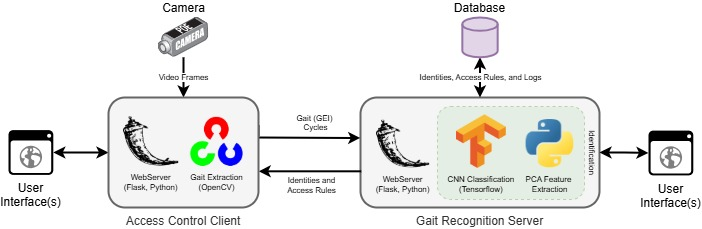
\includegraphics[width=0.9\linewidth]{assets/tech-arch}
    \caption{System Architecture and Technologies}
    \label{fig:system-architecture}
\end{figure}

The Flask web framework is used on both the \ac{acc} and \ac{grs} to render the \ac{ui} and serve \ac{api} endpoints.
The \ac{acc} receives camera input and employs \ac{cv} and image processing techniques using the \ac{cv2} Python library to produce \acp{gei}, these are then transmitted to the \ac{grs} which uses \ac{cnn} and \ac{pca} for feature extraction and identity classification. The following sections detail the design of each component.

\subsection{Gait Energy Image Creation}
\label{subsec:gei-creation}

Real-time, appearance-based \ac{gr} requires pre-processing of camera input to create \acp{gei}s which are used for both identity registration and subsequent classification.

Existing research indicates \acp{gei} creation consists of four main steps, performing subject detection, background subtraction, silhouette normalisation, and silhouette averaging.
The GEI creation steps are illustrated below in Figure \ref{fig:gei-creation-process}, followed by a description of each stage.

\begin{figure}[H]
    \centering
    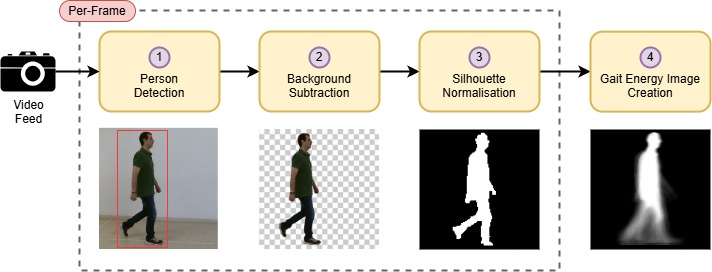
\includegraphics[width=0.9\linewidth]{assets/gei-process.jpg}
    \caption{Steps involved in Gait Energy Image (GEI) Creation}
    \label{fig:gei-creation-process}
\end{figure}

\begin{enumerate}
    \item \textbf{Person Detection}: A person detection algorithm will be used to localise the person present in each given frame. The goal here is to remove any unnecessary parts of the image which may add noise, isolating the subject.
    \item \textbf{Background Subtraction}: The person will be isolated from the remaining background in the frame using statistical differencing (e.g., comparing the frame to a static background), leaving just the subject's silhouette describing their pose at frame $k$.
    \item \textbf{Silhouette Normalisation}: The silhouette image will be normalised to a standard resolution (e.g., 128x88), aligned to the centre of the frame, and given a solid colour to ensure uniformity required for creation of a \ac{gei} with pixel averaging.
    \item \textbf{Silhouette Averaging}: All normalised silhouette images will be combined and averaged using an implementation of $GEI = \frac{1}{N} \sum_{k=1}^{N} I_k$ where $I_k$ is the $k$-th image in the sequence. This results in a grayscale image where pixel intensity (brightness) denotes how often a region was occupied by the subject (a concept outlined in Chapter \ref{chap:context}).
\end{enumerate}

In the final solution, this process will be implemented within the \ac{acc}, where \acp{gei}s will be created and transmitted to the \ac{grs}, which will use the \ac{gei} to either register a new identity, or to perform comparisons to what is stored in the database for identity matching.
However, because of how critical this process is, it will be worked on in isolation before being implemented in a wider context within the \ac{acc}.

\subsection{Access Control Client Design}
\label{subsec:access-control-client-design}

The \ac{acc} will be responsible for processing camera input to create \ac{gei}s that are sent to the \ac{grs} for identity registration or matching.
It will have two main features, listed below, while also allowing asynchronous manual \ac{gei} classification.

\begin{enumerate}
    \item \textbf{Identity Registration}: A 'Save Identity' button can be clicked at any time which will allow the user to assign a label to the current \ac{gei} and send it to the \ac{grs} to be added to the identification model.
    \item \textbf{Person Identification}: Continuously polls the \ac{grs} with updated \ac{gei}s, awaiting a response of the predicted person, confidence score, and access rule.
\end{enumerate}

The \ac{acc} will be controlled using a web-application-based \ac{ui}, allowing the user to view the (1) Live Video Feed, (2) Isolated Silhouette, and (3) Current GEI, in addition to controlling new identity registration.

Fundamentally, the \ac{acc} uses the \ac{gei} creation process defined in Section \ref{subsec:gei-creation} to perform all image processing and averaging actions.

\begin{figure}[H]
    \centering
    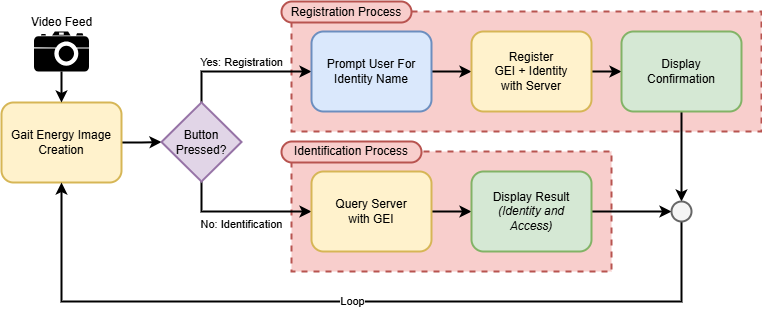
\includegraphics[width=0.9\linewidth]{assets/access-control-client-overview.drawio.png}
    \caption{Access Control Client Features Overview}
    \label{fig:access-control-client-overview}
\end{figure}

Figure \ref{fig:access-control-client-overview} above provides an overview of the \ac{acc} and its two main features, discussed further in the following sections.

\subsubsection{Identity Registration Process}
\label{subsubsec:client-identity-registration}

The \ac{acc} registration process will allow new \ac{gei}s to be stored, enabling subsequent identification.
It will use the same frame buffering and \ac{gei} creation process as Section \ref{subsec:gei-creation}, but will allow the user to assign a label (e.g., name) to the \ac{gei} through the \ac{ui} before it is sent to the \ac{grs} where feature extraction and classification model training will take place.

A sequence diagram, Figure \ref{fig:access-control-client-registration-sequence} below, illustrates the flow of data when a user is registering a new, or updating an existing identity with a new \ac{gei}.

\begin{figure}[H]
    \centering
    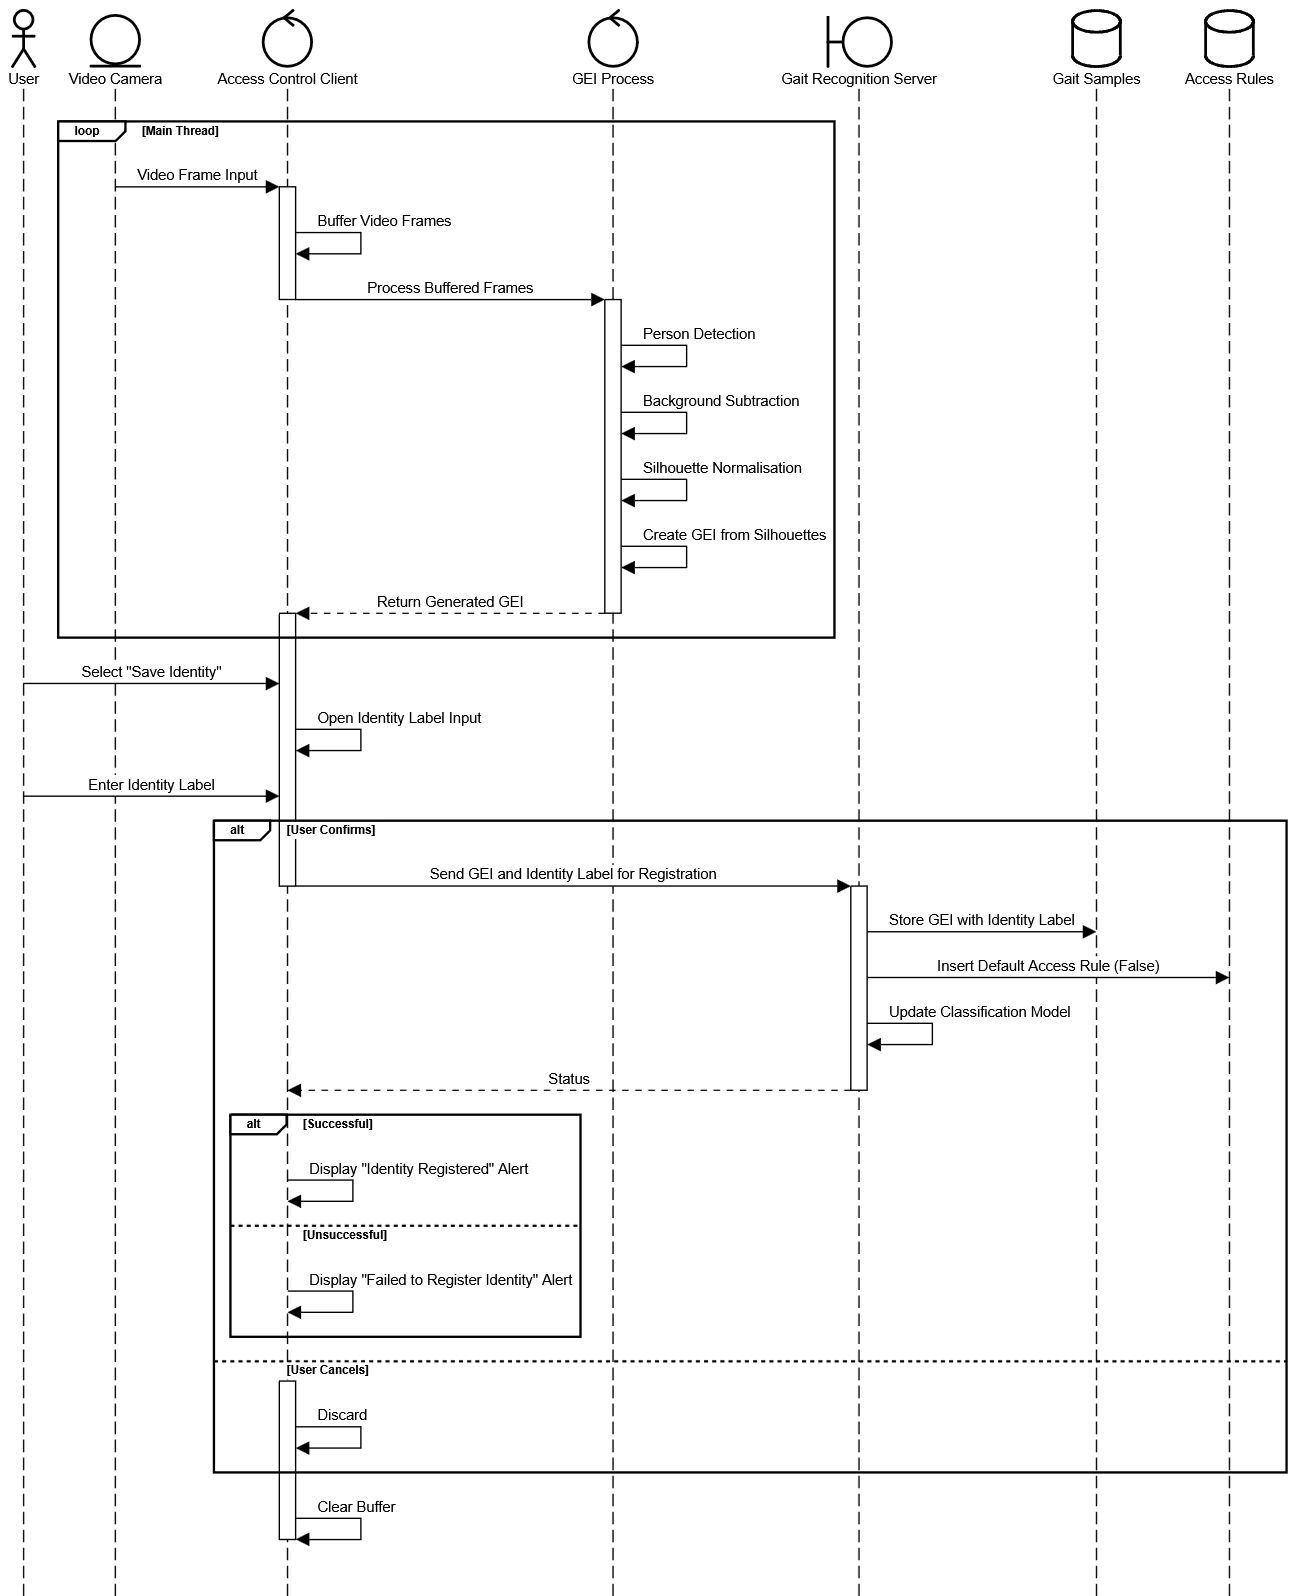
\includegraphics[width=0.65\linewidth]{assets/client-registration-process.png}
    \caption{Access Control Client Registration Process Sequence Diagram}
    \label{fig:access-control-client-registration-sequence}
\end{figure}

\subsubsection{Identity Classification Process}
\label{subsubsec:person-identification}

The \ac{acc} classification will involve cyclically buffering an amount of camera frames before using them to create a \ac{gei} which is sent to the \ac{grs} for classification.
The \ac{acc} will await a response containing a prediction of the identity, confidence score, and access rule. It will display a permit or deny message based on the access rule, \textit{given the confidence score is also above a set threshold}.

A sequence diagram, Figure \ref{fig:access-control-client-identification-sequence} below, illustrates the flow of data from the perspective of the \ac{acc}'s classification thread;
showing the actions performed to transform camera input into \ac{gei}s, and queries made to the \ac{grs} in an attempt to discern identity, as well as the \ac{grs}'s interactions with relevant tables in the database.

\begin{figure}[H]
    \centering
    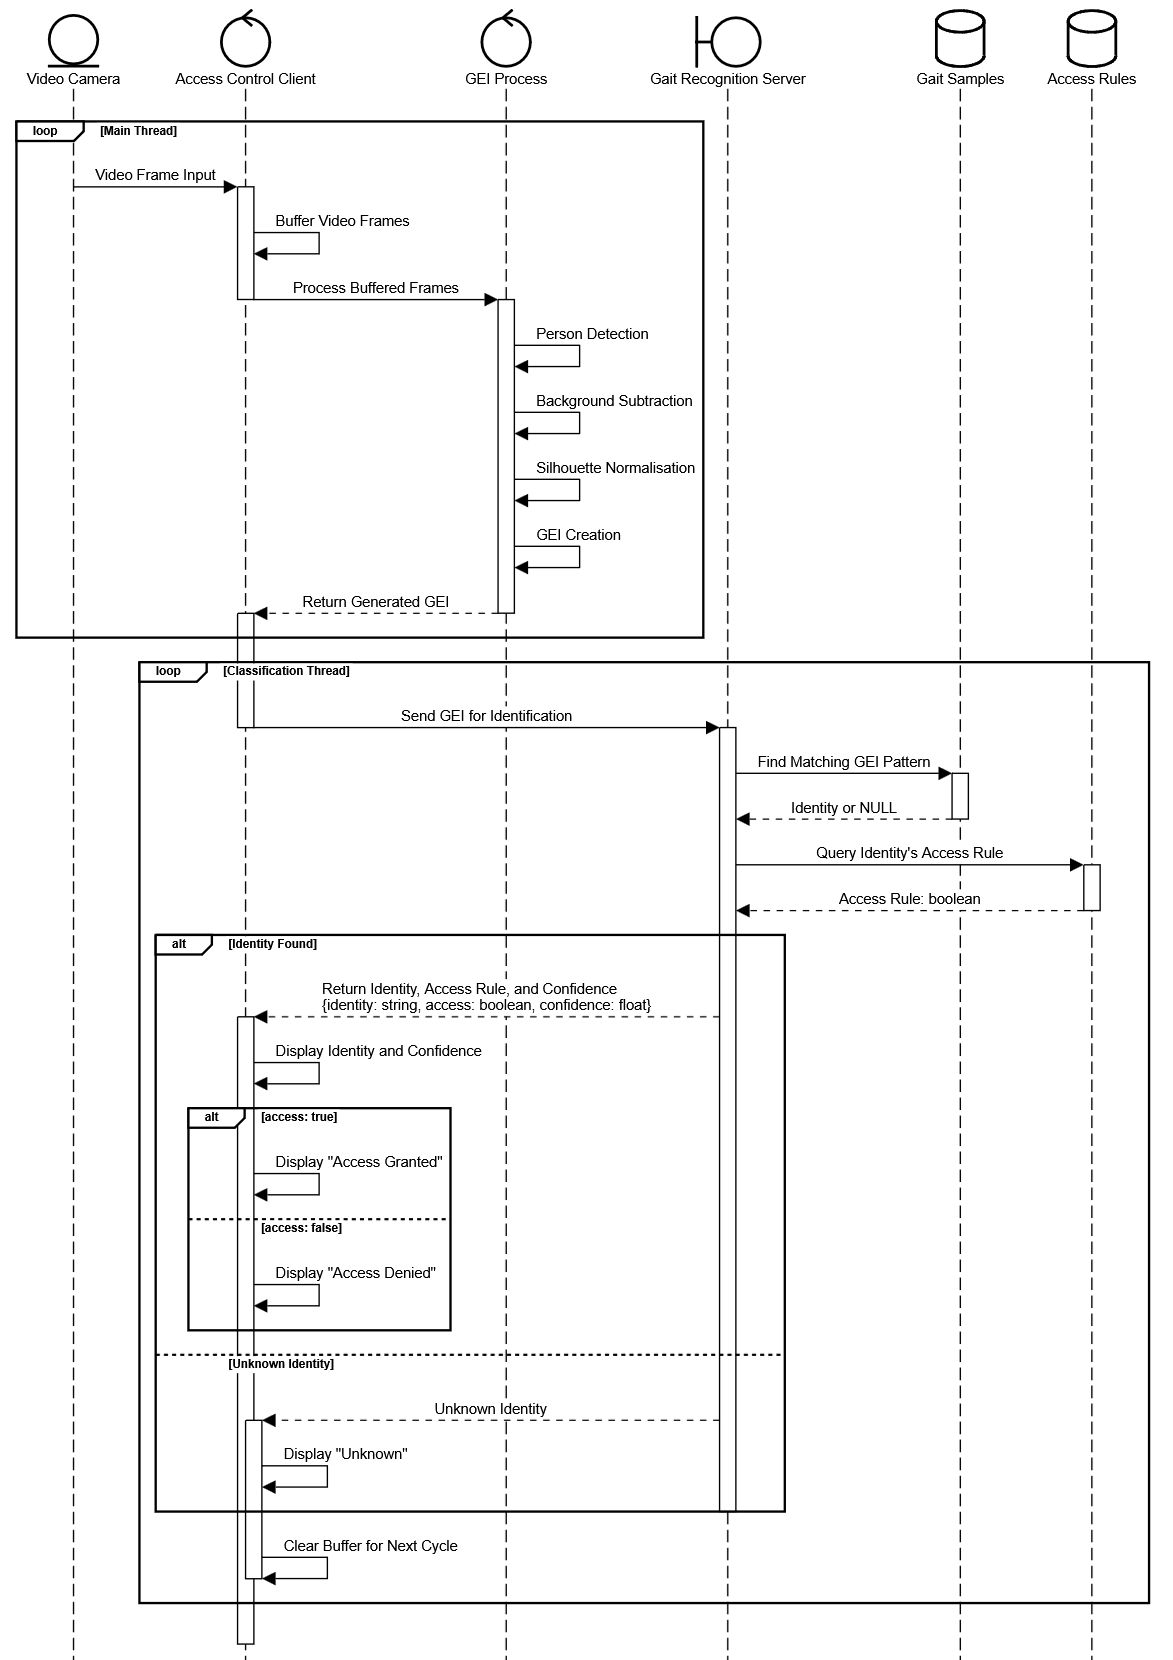
\includegraphics[width=0.65\linewidth]{assets/client-classification-process.png}
    \caption{Access Control Client Identification Process Sequence Diagram}
    \label{fig:access-control-client-identification-sequence}
\end{figure}

This diagram shows:
(1) The \ac{acc} receiving the camera feed input, proceeding to
(2) buffer a number of frames before using them to generate a \ac{gei} with the process defined in Section \ref{subsec:gei-creation}. After the \ac{gei} is created,
(3) the \ac{grs} is queried which
(4) performs classification of the given \ac{gei} and returns the resulting identity or a message stating an identity could not be determined.
If an identity is received,
(5) the \ac{acc} displays the identity label (i.e., the person's name) and uses the Boolean 'access' parameter to display either access granted or denied, if the prediction confidence is above a set threshold.
Finally,
(6) the buffer is cleared and the process repeats, occurring indefinitely until the application is stopped.

Inter-process messaging is to be performed following \ac{rest} principles using \ac{http} (predominantly POST) requests.
Image data is to be encoded prior to transmission in a common format (Base64) allowing serialisation for inclusion in \ac{json} objects.
All messages are to be sent in the \ac{json} format.

\subsubsection{User Interface Design}
\label{subsubsec:client-ui-design}

The \ac{acc}'s \ac{ui} will be a simple, two-page web-application.
The default view, shown in Figure \ref{fig:access-control-client-ui-default-view} below, will display the live camera feed, alongside the isolated silhouette, and the most recently created \ac{gei}.
Underneath these views will be text displaying the label of the most recently identified person, the identification confidence percentage, and a Boolean access rule (set False if confidence is below a set threshold, otherwise respective of the configured access rule).
For refined control, buttons will exist to reset the background image used for background subtraction, and to register the current \ac{gei} to an identity (discussed in Section \ref{subsubsec:client-identity-registration}).

\begin{figure}[H]
    \centering
    \begin{minipage}{0.48\textwidth}
        \centering
        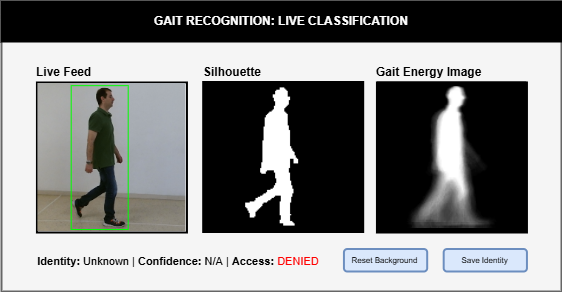
\includegraphics[width=\linewidth]{assets/access-control-client-page-1.drawio.png}
        \subcaption{Default View}
    \end{minipage}
    \hfill
    \begin{minipage}{0.48\textwidth}
        \centering
        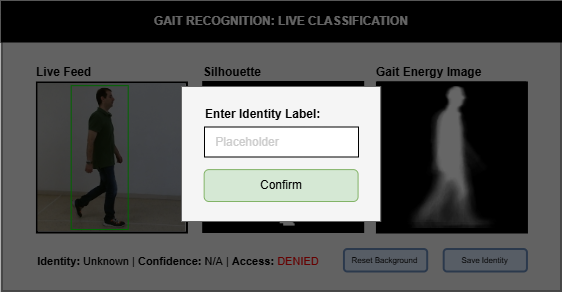
\includegraphics[width=\linewidth]{assets/access-control-client-page-3.drawio.png}
        \subcaption{Label Input Prompt}
    \end{minipage}
    \caption{Access Control Client 'Live Classification' Page}
    \label{fig:access-control-client-ui-default-view}
\end{figure}

The second \ac{acc} page will allow for manual image uploads which will be sent to the server for classification, using the same process defined in Section \ref{subsubsec:person-identification}.
This is predominantly for demonstration and testing purposes but enables asynchronous \ac{gei} classification.
The concept layout of this page can be seen in Figure \ref{fig:access-control-client-ui-manual-view} below, consisting of a drag-and-drop upload box, a preview of the \ac{gei} being classified, and the same text details as Figure \ref{fig:access-control-client-ui-default-view} above.

\begin{figure}[H]
    \centering
    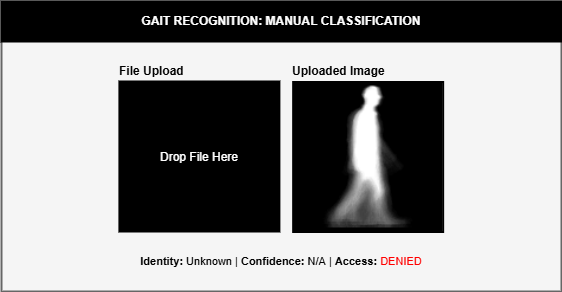
\includegraphics[width=\linewidth]{assets/access-control-client-page-2.drawio.png}
    \caption{Access Control Client 'Manual Classification' Page}
    \label{fig:access-control-client-ui-manual-view}
\end{figure}



\subsection{Gait Recognition Server Design}
\label{subsec:gait-recognition-server-design}

The second component: the \acf{grs}, will be responsible for \ac{gei}-based identity registration and recognition based on input received from the \ac{acc}.
It will also support configuration of Boolean (grant or deny) access control rules tied to each identity, communicated to the \ac{acc} alongside classification results.
The three primary functions of the \ac{grs} are defined below:

\begin{enumerate}
    \item \textbf{Identity Registration}: A new identity is registered by sending a \ac{gei} to the \ac{grs} which will store it in the database.
    \item \textbf{Identity Matching}: A \ac{gei} is sent to the \ac{grs} which will compare it to what is stored in the database, returning a prediction of the identity found, confidence score, and access rule.
    \item \textbf{Access Rule Configuration}: An access rule is configured by sending a request to the \ac{grs} which will update the rule (linked to an identity) in the database.
\end{enumerate}

This component will be controlled using a web-application-based \ac{ui}, enabling configuration of access control rules and a visualisation of registered identities and their associated GEIs (see Section \ref{subsubsec:server-ui-design}).
A \ac{ui} is not required for the \ac{gei}-based registration and matching features as their purpose is to operate continuously in the background and will be accessible to the client via \ac{api} endpoints.

\subsubsection{Identity Registration Process}
\label{subsubsec:server-identity-registration}

The \ac{grs}' identity registration process will support the \ac{acc}'s process defined in Section \ref{subsubsec:client-identity-registration};
awaiting registration messages containing a \ac{gei} and an identity label specified by the user.
No additional image processing will be required here, and the provided \ac{gei} will be stored in the \ac{grs}' database alongside the identity label (e.g., person's name).

A sequence diagram has been used to communicate the flow of data between the \ac{acc} and \ac{grs} when an identity is being registered, shown in Figure \ref{fig:server-identity-registration-sequence} below.

\begin{figure}[H]
    \centering
    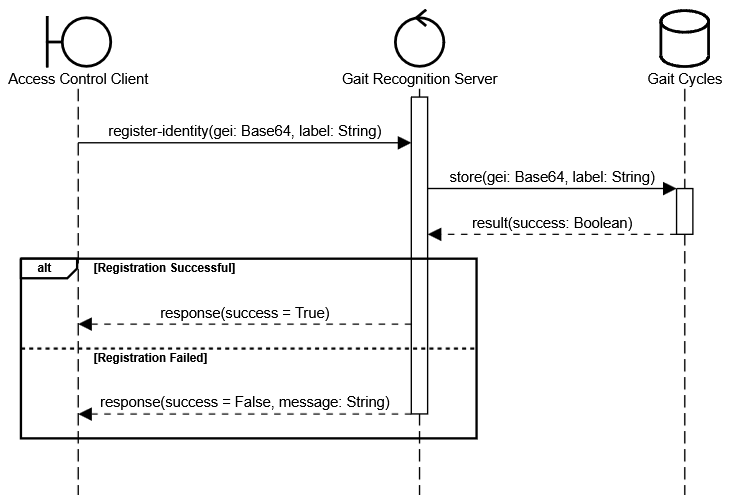
\includegraphics[width=0.65\linewidth]{assets/server-registration-process.png}
    \caption{Server Identity Registration Process Sequence Diagram}
    \label{fig:server-identity-registration-sequence}
\end{figure}

This sequence diagram shows:
(1) a message being received from the \ac{acc} on the 'register-identity' endpoint containing a \ac{gei} and identity label, followed by
(2) the \ac{grs} storing the \ac{gei} and identity label in the gait database, and
(3) the \ac{grs} giving a dynamic response to the \ac{acc} based on whether the identity was successfully registered.

\subsubsection{Identity Classification Process}
\label{subsubsec:identity-matching}

The \ac{grs}' classification process will require no direct interaction from the user.
It will be accessible to the \ac{acc} on an \ac{api} endpoint, allowing the \ac{acc} to send classify messages at set intervals (e.g., every $k$ number of frames) containing the \ac{gei} created with the most recent $k$ frames captured.
The \ac{grs} will then use its classification algorithm to compare the provided \ac{gei} with what is stored in the database, returning the predicted identity, confidence score, and associated access rule.

A sequence diagram has been used to communicate the flow of data between the \ac{acc} and \ac{grs} when gait cycle information is being submitted for identification, shown in Figure \ref{fig:server-identity-classification-sequence} below.

\begin{figure}[H]
    \centering
    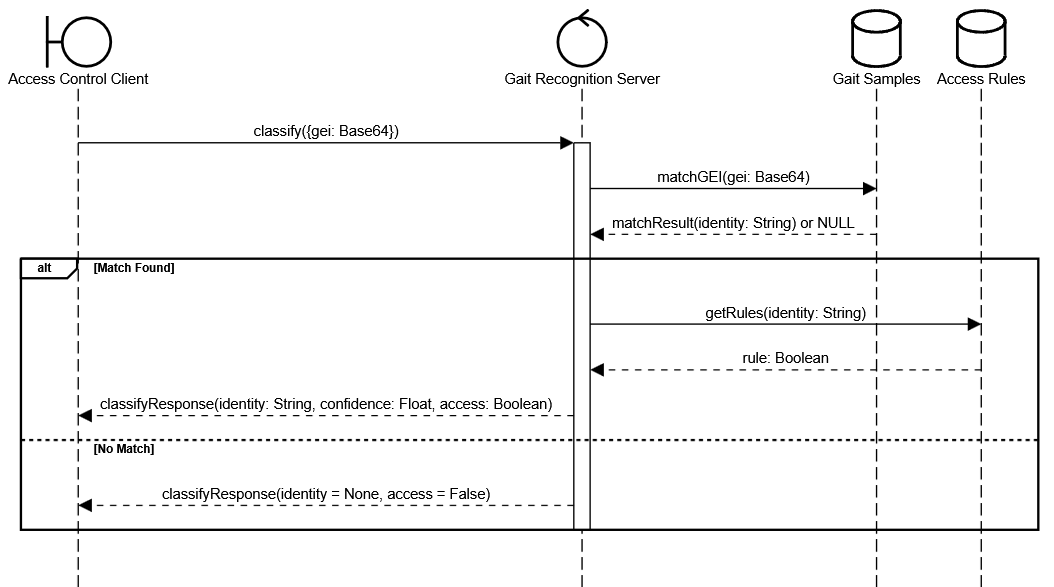
\includegraphics[width=0.65\linewidth]{assets/server-classification-process.png}
    \caption{Server Identity Classification Process Sequence Diagram}
    \label{fig:server-identity-classification-sequence}
\end{figure}

This sequence diagram shows:
(1) a message being received from the \ac{acc} on the 'classify' endpoint containing a \ac{gei}, followed by
(2) the \ac{grs} calling its classification algorithm to find a matching identity, and
(3) the \ac{grs} responding with the matching identity, confidence score, and associated access rules.


\subsubsection{Access Rule Configuration Process}
\label{subsubsec:access-rule-config}

Most user interaction on the server side will occur when viewing existing identities and configuring their associated access control rules (see Section \ref{subsubsec:server-ui-design}).
Users will be able to view the list of registered identities and select any from the list to view the associated \ac{gei}s and access rule configuration.
From there, they will be able to modify the identity's access, with the configuration stored in the access rule table within the database, or delete the identity or individual \ac{gei}s.

The sequence diagram shown in Figure \ref{fig:server-access-rule-configuration-sequence} below illustrates the procedures that will be executed when a user selects an identity from the list, and when they submit a request to update the identity's associated access rule.

\begin{figure}[H]
    \centering
    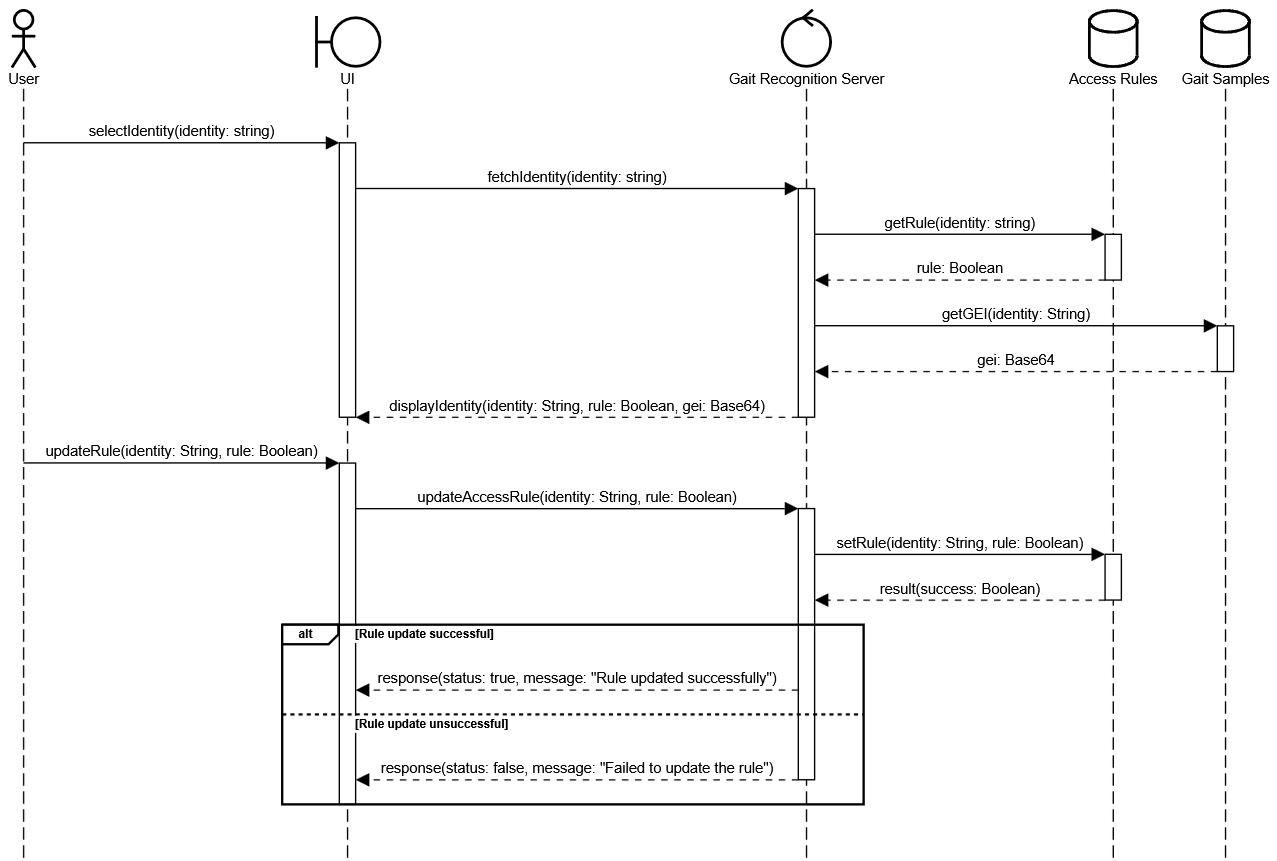
\includegraphics[width=0.65\linewidth]{assets/server-access-rule-management.png}
    \caption{Server Access Rule Configuration Process Sequence Diagram}
    \label{fig:server-access-rule-configuration-sequence}
\end{figure}

\subsubsection{Database Design}
\label{subsubsec:database-design}

The database for the \ac{grs} will enable storage of identites, \ac{gei} samples, access control rules, activity logs, and a trained classification model --- all stored in their own respective tables and linked through relationships where necessary. The following \ac{erd} in Figure \ref{fig:database-erd} illustrates the relationships between these tables:

\begin{figure}[H]
    \centering
    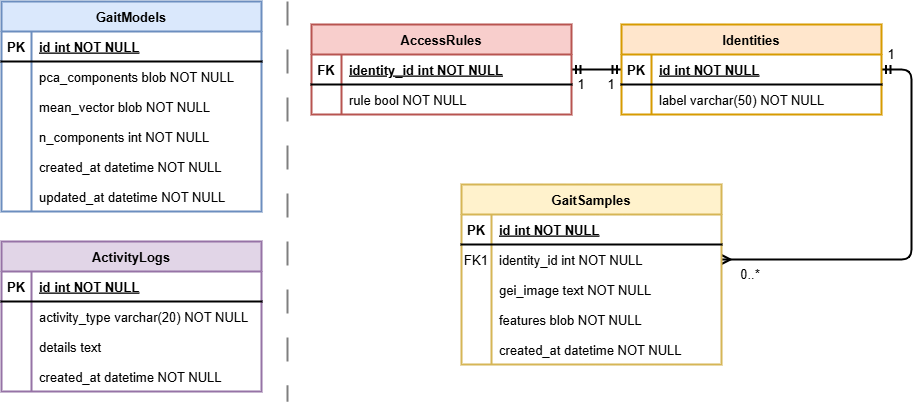
\includegraphics[width=0.9\linewidth]{assets/database-erd.drawio.png}
    \caption{Server Database Entity Relationship Diagram}
    \label{fig:database-erd}
\end{figure}

\paragraph{Identity} Registered identities will be stored in this table, each with a unique identifier and a label (e.g., name). Each identity can have multiple \ac{gei} samples associated with it, with each sample linked to a specific identity through the \codeword{identity\_id} field. A one-to-one relationship will also exist between identities and access rules, with each identity having a single Boolean access rule.

\paragraph{GaitSample} \ac{gei} samples will be stored in this table, each associated with an identity through the \codeword{identity\_id} field. GaitSample table entries will also store the \ac{gei} image as Base64 encoded data, and features extracted from the \ac{gei} as binary data, while also storing the timestamp of when the sample was created.

\paragraph{AccessRule} Boolean access control rules will be stored in this table, each record linked to an identity through the \codeword{identity\_id} field. The \codeword{rule} field will store the Boolean value indicating whether access is granted (\codeword{True}) or denied (\codeword{False}).

\paragraph{GaitModel} A trained classification model will be stored in this table, containing the \codeword{pca\_components} and \codeword{mean\_vector} which will be regularly updated as new \ac{gei} samples are added to the database. The model will be stored as binary data, with the timestamp of when the model was created or last updated also being stored. The model will be used to perform classification on submitted \ac{gei}s as defined in Section \ref{subsubsec:person-identification}.

\paragraph{ActivityLog} System activity history will be stored in this table, including the type of activity, timestamp of when the activity occurred, and dynamic details about the activity (e.g., identity label, access rule, confidence score).

This database design ensures the \ac{grs} can efficiently manage identities, \ac{gei} samples, access control rules, logging, and a classificaiton model in the same place. The relationships defined between tables will also ensure referential integrity is maintained.


\subsubsection{User Interface Design}
\label{subsubsec:server-ui-design}

The \ac{grs}' \ac{ui} will consist of three pages: a home page, an individual per-identity page, and a statistics and logs page.
The home page, shown in Figure \ref{fig:server-ui-home} below, will display the list of registered identities in a grid, with each identity's name, the most recent \ac{gei} sample. Clicking on an identity card will open the individual identity page for the respective identity.

\begin{figure}[H]
    \centering
    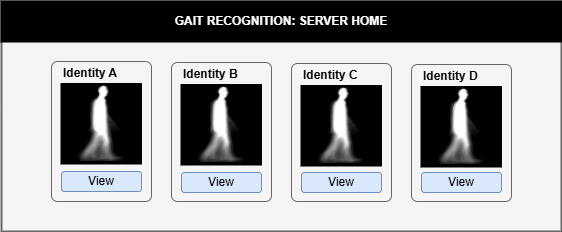
\includegraphics[width=0.9\linewidth]{assets/server-page-1.drawio.png}
    \caption{Gait Recognition Server 'Home' Page}
    \label{fig:server-ui-home}
\end{figure}

The identity page(s), shown in Figure \ref{fig:server-ui-identity} below, will display a selected identity's details, including their label, number of associated \ac{gei} samples, creation date, and a toggleable access control rule. Below this information, a list of the identity's associated \ac{gei} samples will be displayed, each with an global ID number and a button to delete the individual sample.

\begin{figure}[H]
    \centering
    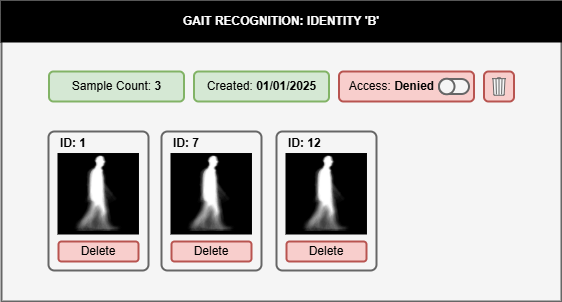
\includegraphics[width=0.9\linewidth]{assets/server-page-2.drawio.png}
    \caption{Gait Recognition Server per-'Identity' Page}
    \label{fig:server-ui-identity}
\end{figure}

Finally, the statistics and logs page, shown in Figure \ref{fig:server-ui-statistics-logs} below, will display the total number of identities registered, the total number of \ac{gei} samples stored, and the average number of \ac{gei} samples per identity. Underneath this information, a chronological list of system activities will be displayed in descending creation order.

\begin{figure}[H]
    \centering
    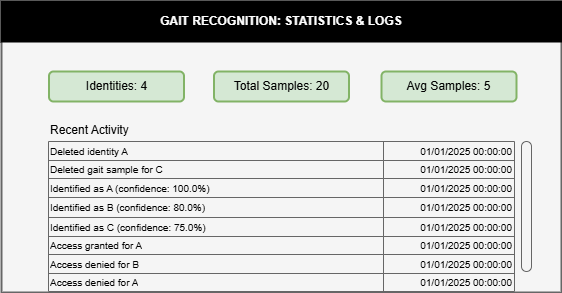
\includegraphics[width=0.9\linewidth]{assets/server-page-3.drawio.png}
    \caption{Gait Recognition Server 'Statistics and Logs' Page}
    \label{fig:server-ui-statistics-logs}
\end{figure}

